
\paragraph{DELETE /:lang/user/:userId}
\begin{itemize}
\item \textbf{Successo} \\
\textbf{Descrizione}:
\label{Procedura di eliminazione account}
\begin{figure}[ht]
	\centering
	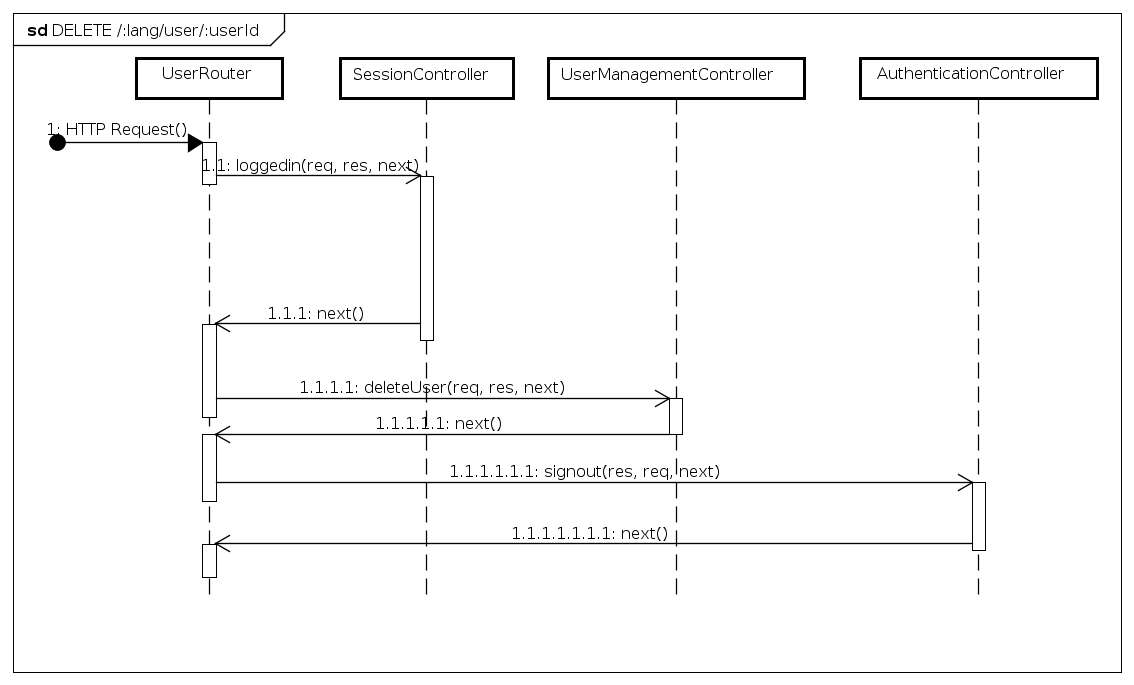
\includegraphics[scale=0.40]{UML/DiagrammiDiSequenza/Back-end/DELETE_LangUserUseridSuccess.png}
	\caption{DELETE /:lang/user/:userId}
\end{figure}

\FloatBarrier

\item \textbf{Fallimento} \\
	\textbf{Descrizione}:
\label{Fallimento della procedura di eliminazione account}
\begin{figure}[ht]
	\centering
	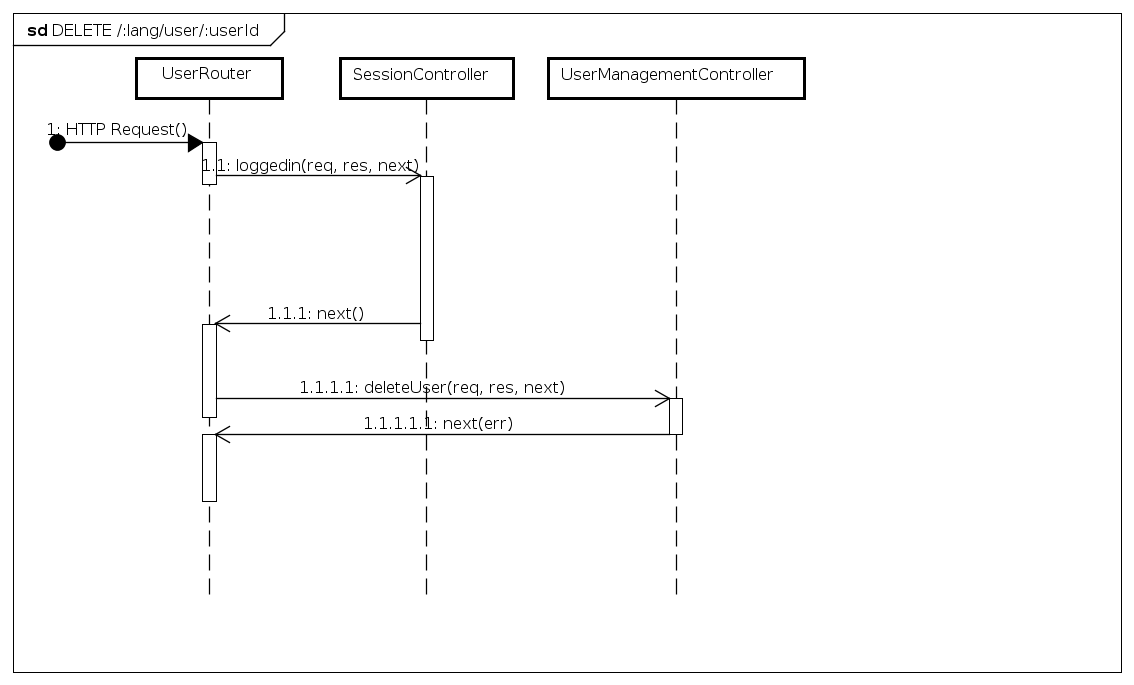
\includegraphics[scale=0.40]{UML/DiagrammiDiSequenza/Back-end/DELETE_LangUserUseridFailure.png}
	\caption{DELETE /:lang/user/:userId}
\end{figure}

\FloatBarrier
\end{itemize}

\paragraph{GET /:lang/user/:userId}
\begin{itemize}
\item \textbf{Successo}
\\
\textbf{Descrizione}:
\label{Procedura di visualizzazione dati utente}
\begin{figure}[ht]
	\centering
	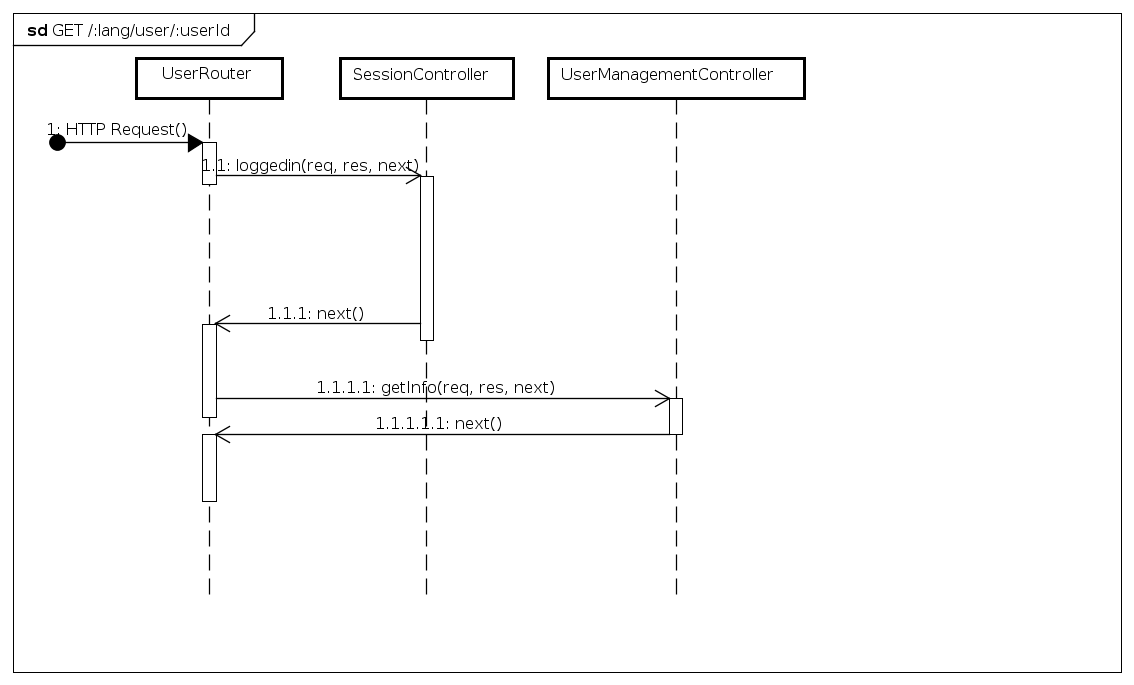
\includegraphics[scale=0.40]{UML/DiagrammiDiSequenza/Back-end/GET_LangUserUserIdSuccess.png}
	\caption{GET /:lang/user/:userId}
\end{figure}

\FloatBarrier

\item \textbf{Fallimento}
\\
\textbf{Descrizione}:
\label{Fallimento della procedura di visualizzazione dati utente}
\begin{figure}[ht]
	\centering
	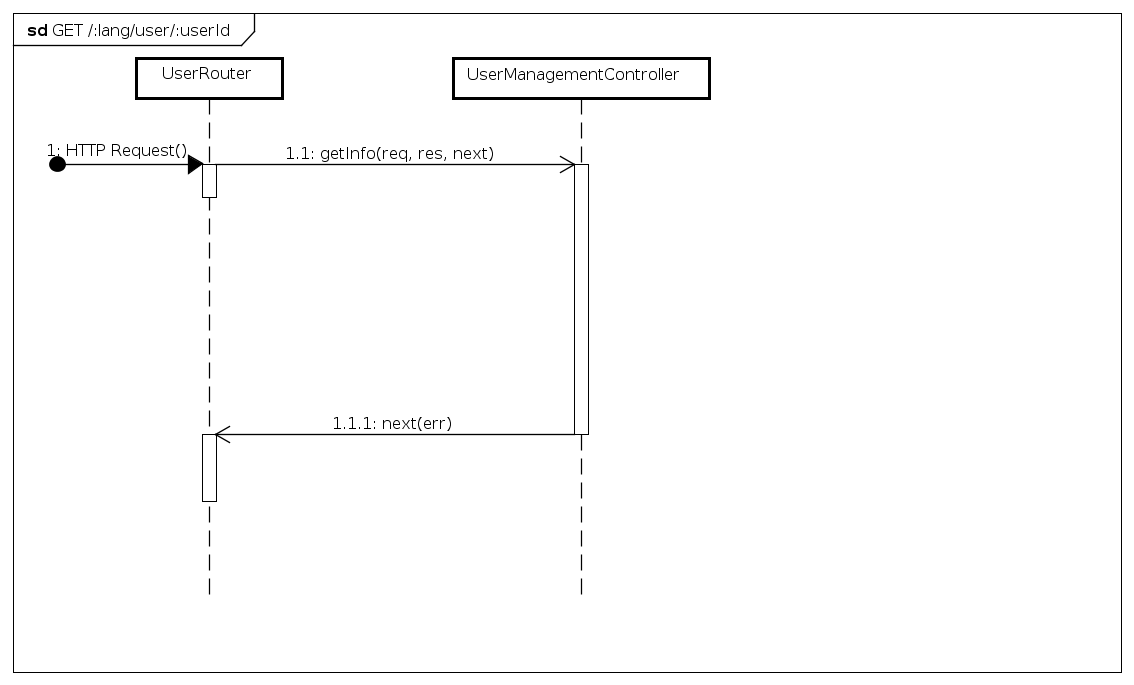
\includegraphics[scale=0.40]{UML/DiagrammiDiSequenza/Back-end/GET_LangUserUseridFailure.png}
	\caption{GET /:lang/user/:userId}
\end{figure}

\FloatBarrier
\end{itemize}

\paragraph{PUT /:lang/user/:userId}
\begin{itemize}
\item \textbf{Successo}
\\
\textbf{Descrizione}:
\label{Procedura di modifica dati utente}
\begin{figure}[ht]
	\centering
	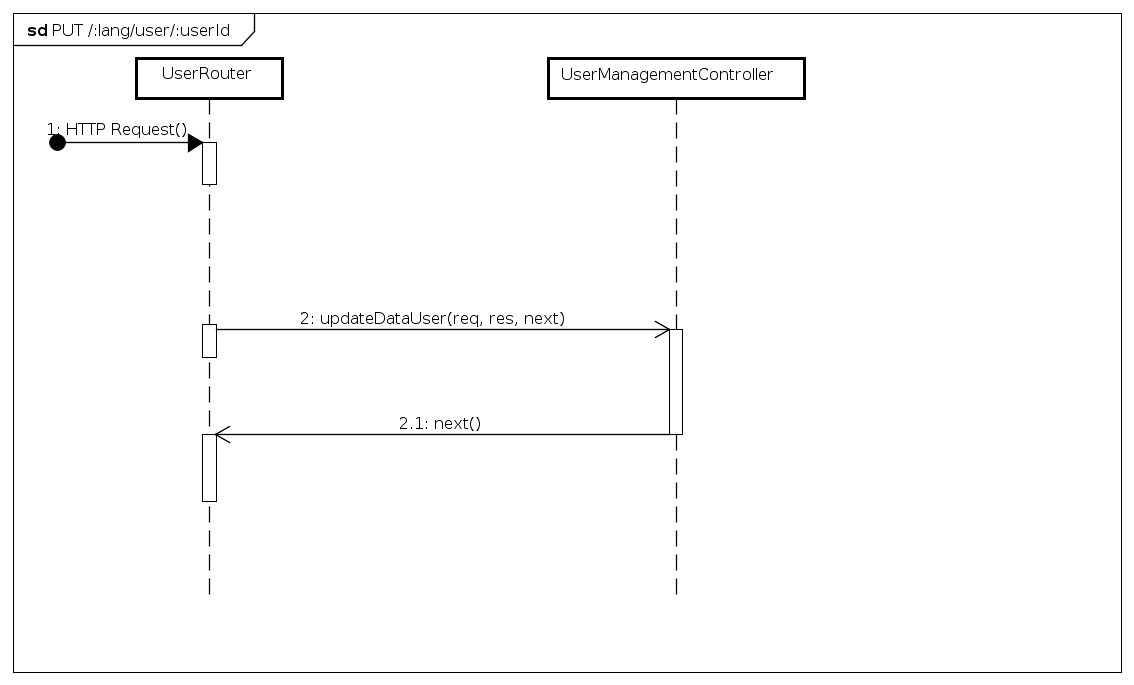
\includegraphics[scale=0.40]{UML/DiagrammiDiSequenza/Back-end/PUT_LangUserUseridSuccess.png}
	\caption{PUT /:lang/user/:userId}
\end{figure}
\FloatBarrier

\item \textbf{Fallimento}
\\
\textbf{Descrizione}:
\label{Fallimento della procedura di modifica dati utente}
\begin{figure}[ht]
	\centering
	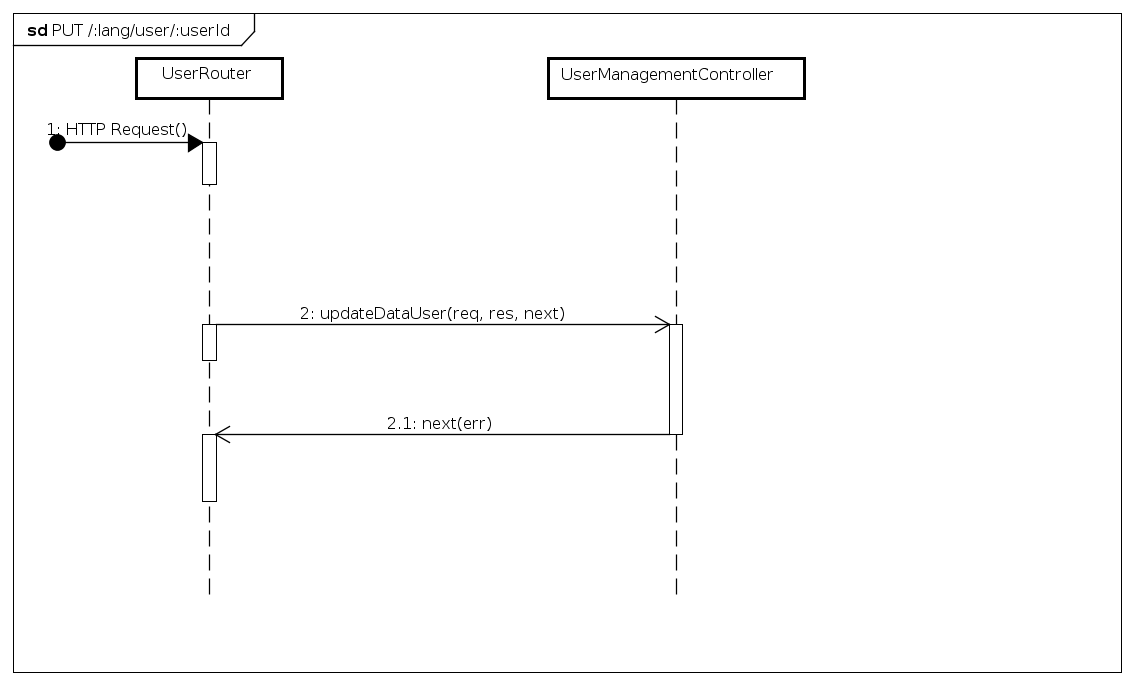
\includegraphics[scale=0.40]{UML/DiagrammiDiSequenza/Back-end/PUT_LangUserUseridFailure.png}
	
	\caption{PUT /:lang/user/:userId}
\end{figure}
\FloatBarrier
\end{itemize}

\paragraph{PUT /:lang/user/:userId/privacy}
\begin{itemize}
\item \textbf{Successo}
\\
\textbf{Descrizione}:
\label{Procedura di modifica password}
\begin{figure}[ht]
	\centering
	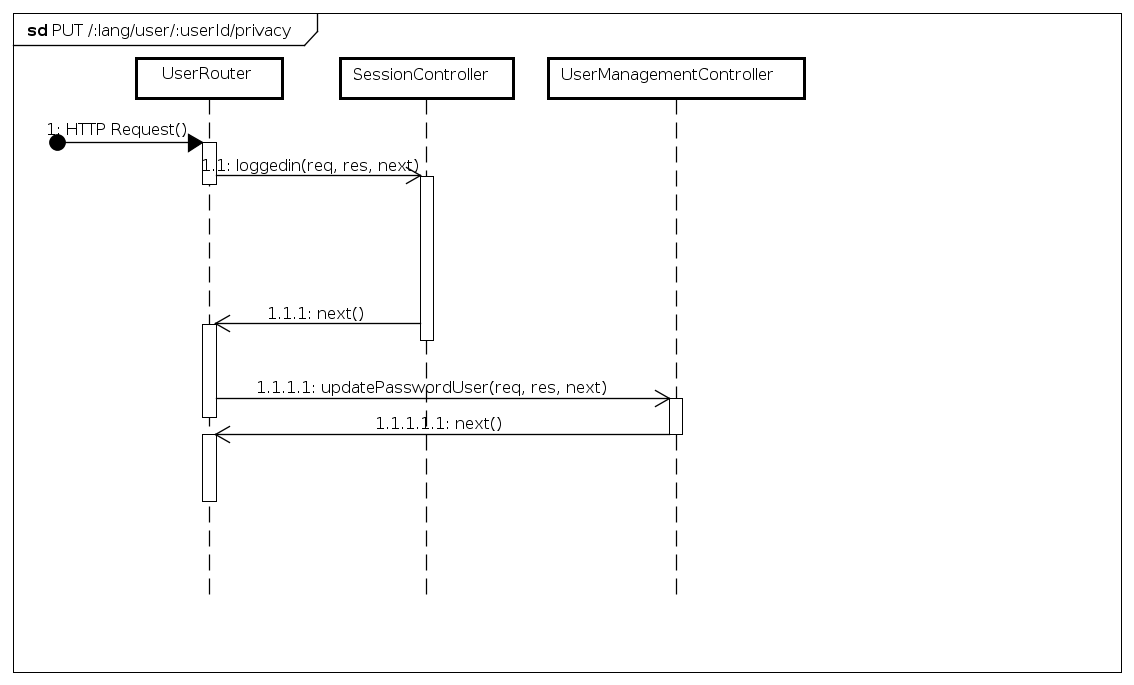
\includegraphics[scale=0.40]{UML/DiagrammiDiSequenza/Back-end/PUT_LangUserUserIdPrivacySuccess.png}
	\caption{PUT /:lang/user/:userId/privacy}
\end{figure}
\FloatBarrier
\item \textbf{Fallimento}
\\
\textbf{Descrizione}:
\label{Fallimento della procedura di modifica password}
\begin{figure}[ht]
	\centering
	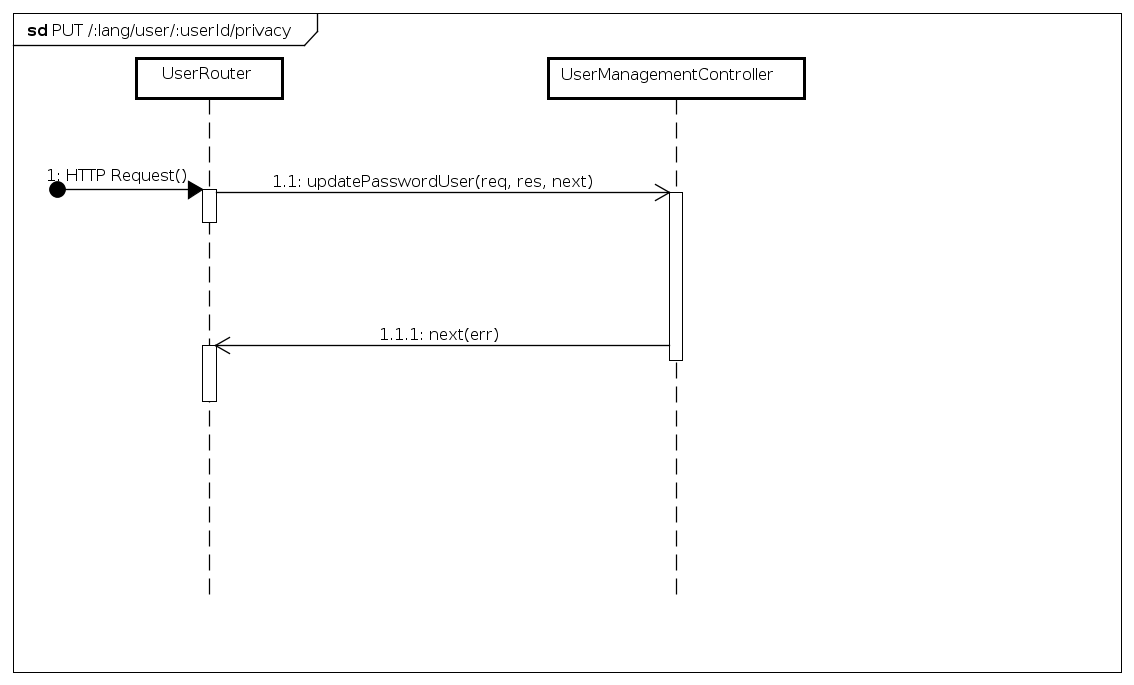
\includegraphics[scale=0.40]{UML/DiagrammiDiSequenza/Back-end/PUT_LangUserUserIdPrivacyFailure.png}	
	\caption{PUT /:lang/user/:userId/privacy}
\end{figure}
\FloatBarrier
\end{itemize}


\paragraph{GET /:lang/user/:userId/statistics}
\begin{itemize}
\item \textbf{Successo}
\\
\textbf{Descrizione}:
\label{Procedura di visualizzazione delle statistiche}
\begin{figure}[ht]
	\centering
	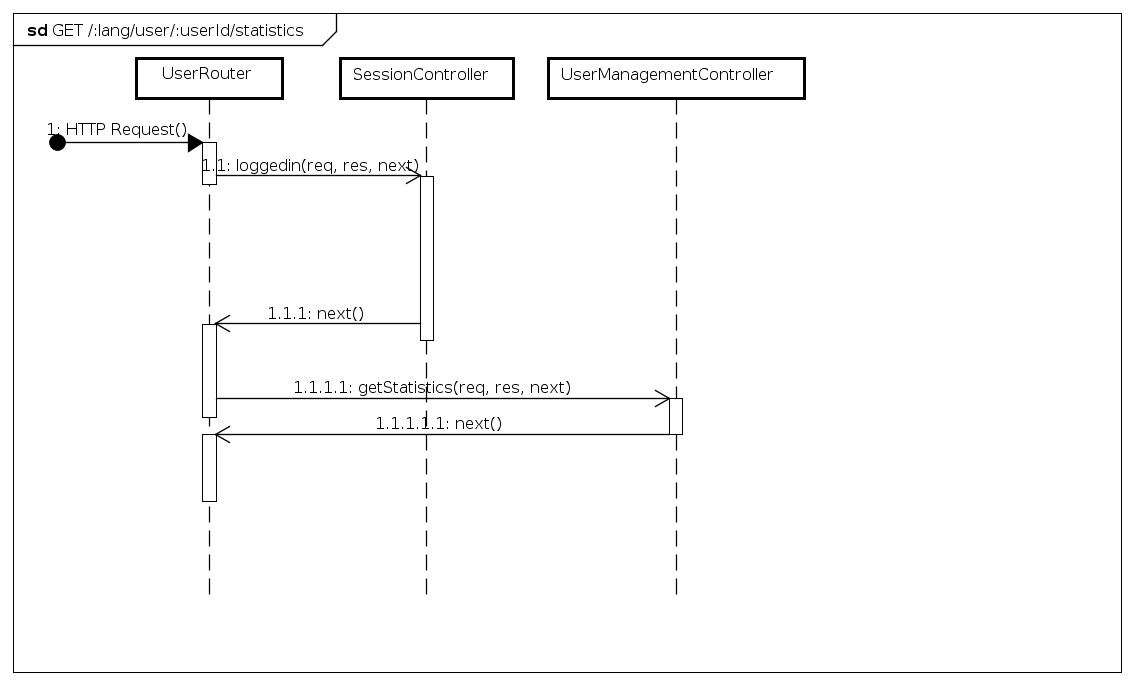
\includegraphics[scale=0.40]{UML/DiagrammiDiSequenza/Back-end/GET_LangUserUserIdStatisticsSuccess.png}
	\caption{GET /:lang/user/:userId/statistics}
\end{figure}
\FloatBarrier
\item \textbf{Fallimento}
\\
\textbf{Descrizione}:
\label{Fallimento della procedura di visualizzazione delle statistiche}
\begin{figure}[ht]
	\centering
	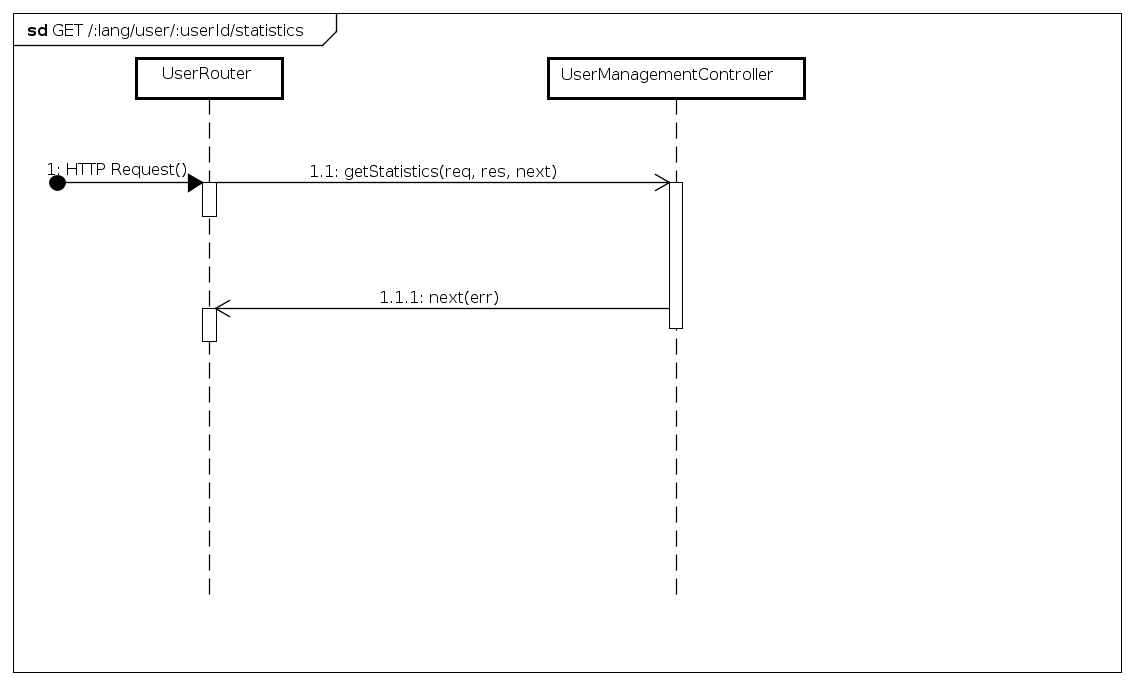
\includegraphics[scale=0.40]{UML/DiagrammiDiSequenza/Back-end/GET_LangUserUserIdStatisticsFailure.png}
	\caption{GET /:lang/user/:userId/statistics}
\end{figure}
\FloatBarrier
\end{itemize}

\paragraph{GET /:lang/user/:userId/statistics/summary/}
\begin{itemize}
\item \textbf{Successo}
\\
\textbf{Descrizione}:
\label{Procedura di visualizzazione della cronologia dei questionari svolti}
\begin{figure}[ht]
	\centering
	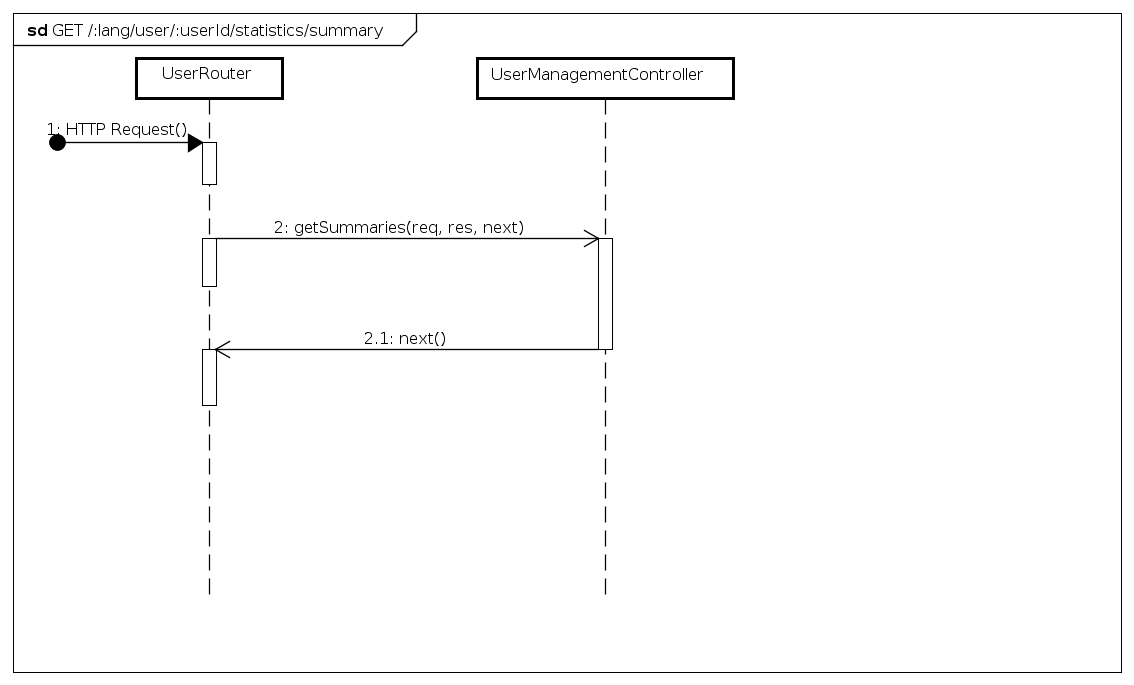
\includegraphics[scale=0.40]{UML/DiagrammiDiSequenza/Back-end/GET_LangUserUserIdStatisticsSummarySuccess.png}
	\caption{GET /:lang/user/:userId/statistics/summary}
\end{figure}
\FloatBarrier
\item \textbf{Fallimento}
\begin{figure}[ht]
	\centering
	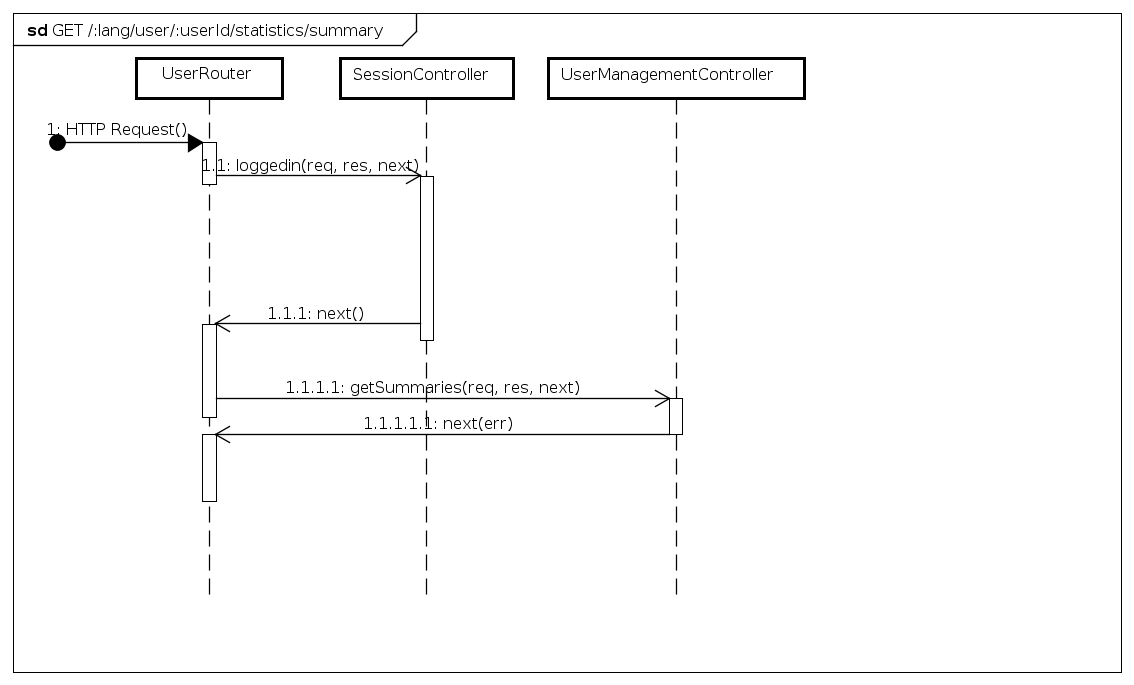
\includegraphics[scale=0.40]{UML/DiagrammiDiSequenza/Back-end/GET_LangUserUserIdStatisticsSummaryFailure.png}
	\caption{GET /:lang/user/:userId/statistics/summary}
\end{figure}
\FloatBarrier

\end{itemize}


\paragraph{GET /:lang/user/:userId/statistics/summary/:summaryId}
\begin{itemize}
\item \textbf{Successo}
% descrizione diagramma e UML
\item \textbf{Fallimento}
% descrizione diagramma e UML
\end{itemize}



